\documentclass[12pt,italian]{report}
\usepackage{tesi}

%
%			INFORMAZIONI SULLA TESI
%			DA COMPILARE!
%

% CORSO DI LAUREA:
\def\myCDL{Corso di Laurea triennale in\\Informatica}

% TITOLO TESI:
\def\myTitle{ANALISI DEI DATI PER PROBLEMI DI MEDICINA LEGALE}

% AUTORE:
\def\myName{Alessandro Beranti}
\def\myMat{Matr. Nr. 855489}

% RELATORE E CORRELATORE:
\def\myRefereeA{Prof. Dario Malchiodi}
\def\myRefereeB{Prof. Anna Maria Zanaboni}

% ANNO ACCADEMICO
\def\myYY{2018-2019}

% Il seguente comando introduce un elenco delle figure dopo l'indice (facoltativo)
%\figurespagetrue

% Il seguente comando introduce un elenco delle tabelle dopo l'indice (facoltativo)
%\tablespagetrue

%
%			PREAMBOLO
%			Inserire qui eventuali package da includere o definizioni di comandi personalizzati
%

% Package di formato
\usepackage[a4paper]{geometry}		% Formato del foglio
\usepackage[italian]{babel}			% Supporto per l'italiano
\usepackage[utf8]{inputenc}			% Supporto per UTF-8
%\usepackage[a-1b]{pdfx}			% File conforme allo standard PDF-A (obbligatorio per la consegna)

% Package per la grafica
\usepackage{graphicx}				% Funzioni avanzate per le immagini
\usepackage{hologo}					% Bibtex logo with \hologo{BibTeX}
%\usepackage{epsfig}				% Permette immagini in EPS
%\usepackage{xcolor}				% Gestione avanzata dei colori

% Package tipografici
\usepackage{amssymb,amsmath,amsthm} % Simboli matematici
\usepackage{listings}				% Scrittura di codice

% Package ipertesto
\usepackage{url}					% Visualizza e rendere interattii gli URL
\usepackage{hyperref}				% Rende interattivi i collegamenti interni

\usepackage{verbatim}

\setcounter{tocdepth}{4}
\setcounter{secnumdepth}{4}
\begin{document}

% Creazione automatica del frontespizio
\frontespizio
\beforepreface

% 
%			PAGINA DI DEDICA E/O CITAZIONE
%			facoltativa, questa è l'unica cosa che dovete formattare a mano, un po' come vi pare
%

{\raggedleft \large \sl Questo lavoro \`{e} dedicato a tutti gli studenti\\
	
	\vspace{2cm}
	
	``Io studio,\\ma studiate pure voi,\\che se studio solo io non serve a un c\dots o''
	
	\bigskip
	
	\--- Gli scarabocchi di Maicol \& Mirco\\
  
	\vspace{2cm}
	
	``No tale is so good \\ that it can't be spoiled \\ in the telling''
	
	\bigskip
	
	\--- Proverbio\\}
         
% 
%			PREFAZIONE (facoltativa)
%

%\prefacesection{Prefazione}
%Le prefazioni non sono molto comuni, tuttavia a volte capita che qualcuno voglia dire qualcosa che esuli dal lavoro in s\'e (come un meta-commento sull'elaborato), o voglia fornire informazioni riguardanti l'eventuale progetto entro cui la tesi si colloca (in questo caso \`e probabile che sia il relatore a scrivere questa parte).

%
%			RINGRAZIAMENTI (facoltativi)
%

\prefacesection{Ringraziamenti}
Questa sezione, facoltativa, contiene i ringraziamenti.

%
%			Creazione automatica dell'indice
%

\afterpreface

% 
%			CAPITOLO 1: Introduzione o Abstract
% 

\chapter{Introduzione}
\label{cap:introduzione}

Questo documento ha una duplice funzione: da un lato mostra un esempio completo di elaborato finale redatto in \LaTeX\ e conforme allo standard PDF/A, e dall'altro contiene suggerimenti e risposte a domande frequenti poste dagli studenti. Se ne raccomanda, pertanto, un'attenta lettura.

\chapter{Machine Learning}
Il termine machine learning, o apprendimento automatico in italiano, si riferisce alla capacità dei computer di apprendere e agire senza essere programmati esplicitamente.
Gli strumenti di machine learning si occupano di dotare i programmi della capacità di "apprendere" e adattarsi agli input forniti
Al giorno d'oggi siamo circondati da tecnologie basate sull'apprendimento automatico:
\begin{itemize}
	\item software che rilevano lo spam a partire dai nostri messaggi e-mail  
	\item i motori di ricerca che imparano a fornirci i migliori risultati possibili
	\item le transazioni con carta di credito sono protette da un software che impara a rilevare le frodi
	\item Le fotocamere digitali imparano a rilevare i volti
	\item le applicazioni di assistenza personale intelligenti sugli smartphone imparano a riconoscere i comandi vocali
	\item addestrare i veicoli per guidare senza assistenza
	\item applicazioni scientifiche come la bioinformatica, la medicina e l'astronomia
\end{itemize}
\section{Come funziona il Machine Learning}
\label{sec:Come funziona il Machine Learning}
Nel Machine learning vengono usati metodi statistici che utilizzano l'esperienza per migliorare le prestazioni di algoritmi o fare previsioni più accurate.
La qualità e la dimensione dei dataset, (collezione di dati), raccolti o resi disponibili utilizzati nel processo sono fondamentali per il successo e l'accuratezza delle previsioni fatte.

Nel processo possiamo distinguere diversi aspetti:
\begin{itemize}
	\item Domain set: raccolta arbitraria di dati, X. Questo è l'insieme di oggetti che si desidera etichettare
	\item Label set: generalmente si usano un set di etichette del tipo \{0, 1\} che rappresentano la presenza o l'assenza della caratteristiche si sta cercando
	\item Training data: è l'input dato in pasto al computer
	\item Algoritmo: scelto in base ai dati in input, è la regola che viene usata dal sistema per classificare e in generale predire la caratteristica
	\item Errore di generalizzazione: è la probabilità che non venga predetta l'etichetta corretta 
\end{itemize}
Una categorizzazione dei compiti del machine learning si ha quando si considera l'output desiderato del sistema che può essere di diversi tipi:
\begin{itemize}
	\item classificazione, i classificatori separano i dati in due o più classi. Quando fornisco un esempio al classificatore, l'algoritmo mi restituisce la classe a cui potrebbe appartenere.
	Esistono due tipi di classificazione:
	\begin{itemize}
		\item binaria, quando le etichette sono soltanto due
		\item multiclasse se le etichette sono tre o più
	\end{itemize}
	\item regressione, usata per predire un valore continuo, per esempio il prezzo di una casa date la dimensione e metratura
	\item clustering, un insieme di input viene diviso in gruppi in modo che i singoli elementi siano simili agli altri punti dello stesso insieme e diversi dagli elementi degli altri. Diversamente da quanto accade per la classificazione, i gruppi non sono noti prima, rendendolo tipicamente un compito non supervisionato.
\end{itemize}
I compiti dell'apprendimento automatico vengono tipicamente classificati in quattro categorie, a seconda della natura del "segnale" utilizzato per l'apprendimento o del "feedback" disponibile al sistema di apprendimento. Queste categorie, anche dette paradigmi, sono:
\begin{itemize}
	\item Machine learning supervisionato
	\item Machine learning non supervisionato
	\item Machine learning per rinforzo
	\item Machine learning semi-supervisionato
	
\end{itemize}

\subsection{Machine Learning con apprendimento supervisionato}
\label{sec:apprendimento supervisionato}
Attravero l’apprendimento supervisionato cerchiamo di costruire un modello partendo da dei dati di addestramento etichettati, con i quali cerchiamo di fare previsioni su dati non disponibili o futuri. Con il termine "supervisione" si intende quindi che nel nostro insieme dei campioni (o dataset), i segnali di output desiderati sono già noti poiché precedentemente etichettati.

Esistono molti algoritmi per svolgere apprendimento supervisionato, durante il tirocinio ho avuto modo di usare:
\begin{itemize}
	\item Support Vector Machine
	\item Decison Tree Classifier
	\item Random Forest Classifier
	\item Gaussian Naive Bayes
	\item Linear Discriminant Analysis
	\item Multi-Layer Perceptron Classifier
\end{itemize}

\subsubsection{Support Vector Machine}
\label{sec:SVC}
Il Support Vector Machine è un algoritmo di apprendimento automatico supervisionato che può essere usato sia per scopi di classificazione che di regressione, ha la sua massima efficacia in problemi di classificazione binaria anche se può essere utilizzato anche per problemi di classificazione multiclasse.

L'SVM è basato sull'idea di riuscire a trovare un iperpiano che divida al meglio un set di elementi in due classi distinte, definiamo alcuni concetti chiave:
\begin{comment}
\begin{figure}[b]
\centering
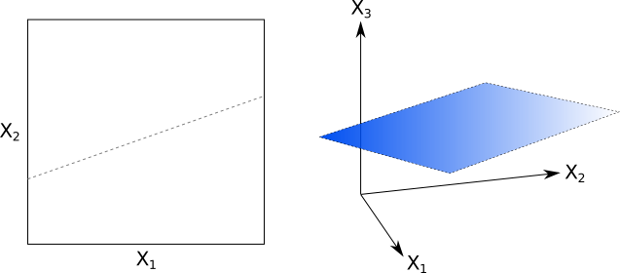
\includegraphics[width = 60mm]{immagini/Iperpiano-3-dimensioni}
\caption{Il processo di trasformazione delle idee in testo~\cite{hamalainen2019web}.}
\label{fig:ideas2text}
\end{figure}
\begin{figure}[b]
\centering
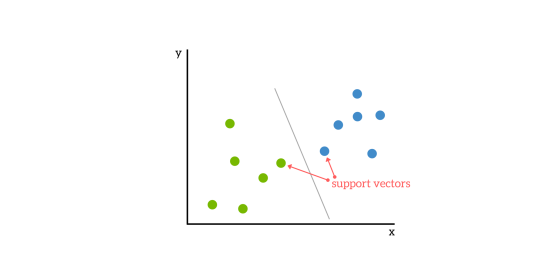
\includegraphics[width = 100mm]{immagini/support_vector}
\caption{Il processo di trasformazione delle idee in testo~\cite{hamalainen2019web}.}
\label{fig:ideas2text}
\end{figure}
\end{comment}


\begin{itemize}
	\item Iperpiano: nel caso in cui sia abbiano solo due dimensioni spaziali $x_1$ e $x_2$, l'iperpiano è raffigurato come una linea che separa un insieme di dati. Nel caso in cui le dimensioni siano 3, l'iperpiano è raffigurato come un piano, vedi immagine 1.
	Con più di 3 dimensioni viene definito "iperpiano".
	\item Support Vector: chiamati vettori di supporto in italiano, sono i punti che si trovano piu vicini all'iperpiano che divide i dati.
	\item Margine: è la distanza tra i vettori di supporto di due classi diverse. A metà di questa distanza viene tracciato l'iperpiano. (immagine da inserire)
\end{itemize}

Il Support Vector Machine ha l'obiettivo di identificare l'iperpiano che divide meglio i vettori di supporto in classi, per fare ciò esegue due step:

\begin{itemize}
	\item Cerca un iperpiano linearmente separabile che separa i valori di una classe dall'altra. Nel caso in cui ne esista più di uno cerca quello con il margine più alto tra i vettori di supporto in modo da migliorare l'accuratezza del modello
	\item se l'iperpiano cercato non esiste, Support Vector Machine usa una mappatura non lineare per trasformare i dati di allenamento in una dimensione superiore. In questo modo, i dati di due classi possono sempre essere separati da un iperpiano, che sarà scelto per la suddivisione dei dati.  
\end{itemize}

Un iperpiano linearmente separabile è un iperpiano in cui è semplice distinguere due classi. Nella seguente immagine è visibile come sia possibile disegnare un numero infinito di linee rette per separare i diversi elementi. Il problema è trovare quale tra le infinite rette risulti ottimale, ossia quella che generi il minimo errore di classificazione su una nuova osservazione.
Per fare ciò dobbiamo avere i nostri elementi il più lontano possibile dal iperpiano pur rimanendo nella zona corretta. (immagine linearmente separabili)

Nel momento in cui vengono aggiunti nuovi dati di test, il modello decide la classe che gli appartiene. (allego foto con esempio massimizzato)

Dato un training set etichettato:

\begin{center}
	\[
	\ (x_1, y_1), ..., (x_n, y_n) \in R^{d} and 
	\ y_i \in (-1, +1)
	\]
\end{center}
dove $x_i$ sono le dimensioni del vettore e $y_i$ sono le etichette.

L'iperpiano ottimale è definito come 
\begin{center}
	\[w_0 + w_1x_1 + w_2x_2 +...+ w_nx_n= 0\]
\end{center}
dove w è il vettore di peso, x è il vettore di caratteristiche di input e $w_0$ è il bias.
In sostanza in $n$ dimensioni un iperpiano di separazione è una combinazione lineare di tutte le dimensioni uguagliate a 0.
Ragionando a due dimensioni per semplificare il problema abbiamo che 
\begin{center}
	\[w_0 + w_1x_1 + w_2x_2 = 0\]
\end{center}
I punti che stanno sopra l'iperpiano , e che rappresentano un classe , soddisfano la seguente condizione:
\begin{center}
	\[w_0 + w_1x_1+w_2x_2 > 0\]
\end{center}
mentre qualsiasi punto che si trova sotto l'iperpiano, appartiene all'altra classe, che è soddisfatta dalla seguente condizione 
\begin{center}
	\[w_0 + w_1x_1+w_2x_2 < 0\]
\end{center}
Includendo anche i limiti dei margini delle classi si hanno le seguenti condizioni:
\begin{center}
	\[w_0 + w_1x_1+w_2x_2 \geq 1,
	\ if
	\ y=1\]
	\[
	\ w_0 + w_1x_1+w_2x_2 \leq 1 
	\ if
	\ y = -1
	\]
	\[ y \in (-1, +1)\]
\end{center}
Se il vettore dei pesi è indicato da $w$ e $\parallel w \parallel$ è la sua lunghezza, allora la dimensione del margine massimo è 
\begin{center}
	\[ \frac{1}{\left | w \right |} + \frac{1}{\left | w \right |} = \frac{2}{\left | w \right |}\]
\end{center}
ciè significa cge minimizzando il vettore peso $w$, avremo margine massimo che determina l'iperpiano ottimale.

Non è però sempre possibile dividere i dati tramite un iperpiano, nella figura sotto vi è un chiaro esempio  (allega foto)

Per utilizzare la classificazione tramite iperpiani anche per dati che avrebber bisogno di funzioni non lineari per essere separati, è necessario ricorrere alla tecnica degli spazi immagine ($feature$ $spaces$). Questo metodo, che sta allabase della teoria delle SVM, consiste nel mappare i dati iniziali in uno spaziodi dimensione superiore.  Presupponendo quindi $m > n$, per la mappa si utilizza una funzione
\begin{equation}
	\phi: \mathbb{R}^{n} \rightarrow \mathbb{R}^{m}
\end{equation}
attraverso la funzione $\phi$ i dati vengono mappati in uno spazio in cui diventano linearmente separabili e in cui sarà possibile trovare un iperpiano che li separi.

La tecnica degli spazi immagine è particolarmente interessante per algoritmi che utilizzano i dati di training $x_i$ solo attraverso prodotti scalari $x_i \cdot x_j$. In questo caso nello spazio $\mathbb{R}^{m}$ non si devono trovare esplicitamente $\phi(x_i)$ e $\phi (x_j)$ ma basta calcolare il loro prodotto scalare $\phi (x_i) \cdot \phi (x_j)$. Per rendere semplice questo ultimo calcolo, che in spazi di dimensioni elevate diventa molto complicato, si utilizza una funzione detta kernel che restituisce direttamente il prodotto scalare delle immagini:
\begin{equation}
K(x_i, x_j) = \phi (x_i) \cdot \phi (x_j)
\end{equation}
Esistono svariati kernel, i più utilizzati sono:
\begin{itemize}
	\item Lineare: $K(x, y) = x \cdot y$
	\item Polinomiale: $K(x, y) = (x \cdot y)^{d}$ oppure $K(x, y) = (1 + x \cdot y)^{d}$
	\item Gaussian Radial Basis function: $K(x,y) = exp (- \left | x-y \right |^2)/(2 \sigma 2)$
	\item Sigmoid: $K(x,y) = tanh(k x \cdot y - \delta)$ 
\end{itemize}

\subsubsection{Decision Tree Classifier}
Il Decision Tree Classifier è un algoritmo di apprendimento supervisionato. Utilizza un albero decisionale, decision tree, composto da:
\begin{itemize}
	\item 
\end{itemize}
\subsubsection{Random Forest Classifier}
\subsubsection{Gaussian Naive Bayes}
\subsubsection{Linear Discriminat Analysis}
\subsubsection{Multi-Layer Perceptron Classifier}
\subsection{Machine Learning con apprendimento Non Supervisionato}
Nell’apprendimento senza supervisione, al contrario di quella supervisionata abbiamo dei dati senza etichetta o dati non strutturati. Con queste tecniche siamo in grado di osservare la struttura dei dati e di estrapolare informazioni cariche di significato. In queste tecniche non si può però contare su una variabile nota relativa al risultato o su di una funzione di ricompensa.

Abbiamo due tecniche che ci vengono in aiuto nell’affrontare problemi di apprendimento non supervisionato: il Clustering e la Riduzione della dimensionalità dei dati.
\subsection{Machine Learning con apprendimento per Rinforzo}
Il terzo tipo di apprendimento automatico è l’Apprendimento per Rinforzo. L’obiettivo di questo tipo di apprendimento è quello di costruire un sistema (agente) che attraverso le interazioni con l’ambiente migliori le proprie performance.

Per poter migliorare le funzionalità del sistema vengono introdotti dei rinforzi, ovvero segnali di ricompensa.

Questo rinforzo non è dato dalle label (etichette) o dai valori corretti di verità, ma è una misurazione sulla qualità delle azioni intraprese dal sistema. Per questo motivo non può essere assimilato ad un apprendimento supervisionato.

Attraverso algoritmi che fanno largo utilizzo del Deep Learning, è tornato di moda questo tipo di apprendimento. Potremmo trovare questo tipo di apprendimento ad esempio nell’addestramento di un sistema per il gioco degli scacchi.

Inizialmente le mosse saranno del tutto casuali e senza una logica. Dal momento in cui il sistema riceverà dei feedback positivi, come ad esempio nel caso in cui mangi una pedina avversaria, allora riceverà un peso maggiore e conseguentemente un rinforzo positivo su quell’azione. Contrariamente in caso di azione negativa, il valore dei pesi su quell’azione andrà in decremento.

Conseguentemente a questi rinforzi, il sistema darà maggior peso alle mosse che gli hanno portato maggiori benefici e tenderà a replicare lo stesso comportamento su nuove mosse future.
\subsection{Machine Learning con apprendimento semi Supervisionato}
Può essere visto come un quarto tipo di apprendimento automatico. In questo caso, al contrario dell’apprendimento non supervisionato, abbiamo che di tutti i dati presenti nel training set, solo pochi di essi sono stati etichettati.
% 
%			CAPITOLO 2: Stato dell'arte
% 

\chapter{Dataset}


\section{Iris}


\section{Incidenti Stradali}





\section{Metodi per ridurre la Dimensionalità}



\subsection{PCA}
\subsection{TSNE}


% 
%			CAPITOLO 3: Tecnologie utilizzate
% 

\chapter{Esperimenti}
\label{cap3}



\section{Model Selection}

\subsection{Scelta degli Iperparametri}

\begin{equation}
x_i(n) = a_{i1}u_1(n) + a_{i2}u_2(n) + \cdots + a_{iJ}u_J(n) \, .
\label{eq:multimix}
\end{equation}

\subsection{Scalare i dati}


\section{Errore di Generalizzazione}
\label{sec:errore}


\subsection{Training}



\subsection{Cross Validation}



\section{Risultati Ottenuti}
\label{sec:risultati}


% 
%			CAPITOLO 4: Conclusioni e sviluppi futuri
% 
\section{Conclusioni}

Nelle conclusioni si tirano le somme di quanto realizzato, facendo un riassunto stringato del lavoro svolto. In particolare vanno dichiarati punti di forza e criticità della ricerca effettuata, nonché quali aspetti dello stato dell'arte siano stati superati dal lavoro in oggetto.

%
%			BIBLIOGRAFIA
%

\bibliographystyle{unsrt}
\bibliography{bibliografia}
\addcontentsline{toc}{chapter}{Bibliografia}


% Pagina dichiusura del LIM
\closingpage

\end{document}


 